\section{噪声形成模型}

相机传感器在采集图像时往往不可避免地会产生噪声,采集到的原始图像,即RAW图像,是未经图像信号处理器(Image Signal Processor,ISP)处理的原始信号。由于不同的相机的ISP往往相去甚远,且经ISP处理之后,噪声分布通常会显著改变\cite{noiseflow},本文的工作将主要考虑原始域噪声建模。数字传感器原始图像$I$一般可以表示为干净图像$C$和噪声$N$的总和,表达如下:
\begin{equation}
	I = C + N
\end{equation}

噪声建模的目的是利用统计模型描述噪声$N$的特性。一般来说,噪声$N$的成分很复杂,但可以分为与信号相关的噪声和与信号无关的噪声。
本文采用了上文所介绍过的,Wei等人提出的基于物理的噪声模型ELD\cite{eld},该模型考虑了真实世界噪声中最关键的成分,具有良好的泛化性能。由于ELD模型针对的是暗光条件下噪声的形成,本文将对ELD模型做出一些调整,使之更加泛用。本文所使用的真实世界噪声形成模型可表示为:
\begin{equation}
	N=N_p+N_{read }+N_{row }+N_q
	\label{noisemodel}
\end{equation}

下面本文简要介绍一下上述各噪声成分。

光子噪声$N_p$,是一种与信号相关的噪声,它的形成来自于传感器收集到的光子数量不稳定,这种不稳定性使光子噪声遵循泊松分布\cite{photon},可描述为:
\begin{equation}
	N_p \sim \mathcal{P}(\lambda)
\end{equation}
其中参数$\lambda$表示入射光子的平均数量。

读取噪声$N_{read}$,当电路读取可测量电压并产生随机振动时,就会产生读取噪声。根据ELD模型\cite{eld},在非暗光条件下,读取噪声可以被假定为遵循高斯分布,均值为$\mu_r$,方差为$\sigma_r^2$,进而可以描述为:
\begin{equation}
	N_{\text {read }} \sim \mathcal{N}\left(\mu_r, \sigma_r^2\right) 
\end{equation}

行噪声$N_{row}$,由逐行传感器的读出格式引起,通常建模为零均值高斯分布,方差为$\sigma_{row}^2$:
\begin{equation}
	N_{\text {row }} \sim \mathcal{N}\left(0, \sigma_{row}^2\right) 
\end{equation}

量化噪声$N_q$,当连续模拟信号转换为离散数字值时,量化噪声就会被引入。量化噪声通常被认为服从均匀分布$U$:
\begin{equation}
	N_q \sim U\left(-\frac{1}{2 q}, \frac{1}{2 q}\right)
\end{equation}
其中 $q$ 是量化步骤。

总的来说,噪声模型中需要估计的五个参数是$\boldsymbol{P}=\left(\lambda, \mu_r, \sigma_r, \sigma_{\text {row }}, q\right)$,这些参数共同决定了最终生成的噪声。


\section{基于标准化流模型的噪声参数先验}

\subsection{模型整体框架}

在真实场景下,在RAW图像中捕获到的噪声是复杂的,并且与图像信号有关。现有的使用标准化流的方法\cite{noiseflow, srgbflow},往往直接从基础分布中生成噪声,这就带来了两个问题:

(1) 它们需要大量成对的噪声-干净图像数据集来获得真实的噪声。

(2) 从简单分布到真实噪声的训练过程不稳定,尤其是在光线不足的条件下\cite{srgbflow,ftd}。

为了提高噪声建模的准确性,本文使用标准化流模型来生成噪声参数,而不是噪声本身。具体来说,本文的工作通过标准化流模型,在噪声参数和高斯分布之间建立一个双射映射。本文所提出的噪声参数流模型架构如图\ref{fig:parameterflow}所示。

\begin{figure}[h]
	\centering
	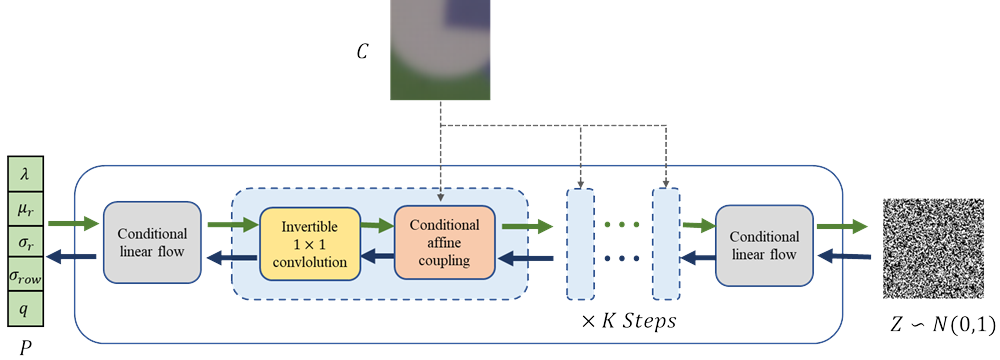
\includegraphics[width=1.0\textwidth]{imgs/parameterflow.pdf}
	\caption{本文提出的用于生成噪声参数的标准化流模型结构。}
	\label{fig:parameterflow}
\end{figure}

给定一个观测到的干净图像数据集$\mathcal{C}=\left\{C_i\right\}_{i=1}^M$和相应的校准噪声参数$\mathcal{P}=\left\{\boldsymbol{P}_i\right\}_{i=1}^M$,其中$M$是数据集的大小。噪声参数$\boldsymbol{P}_i$首先通过条件线性流(Conditional Linear Flow,CLF)层映射为线性变换。在随后的模型中,可逆的$1\times1$卷积层和条件仿射耦合(Conditional Affine Coupling,CAC)层交替使用$K$次。其中,干净的图像作为条件信息进入CAC层作为条件信息。详细的流模型结构将会在下文叙述。模型最后得到的$z$是一个服从标准高斯分布的分布。

上文所叙述的噪声参数流模型可以用式\ref{nllloss}中的负对数似然损失函数进行训练。本文所提出的技术可视为基于流模型的噪声参数先验,它利用标准化流模型的生成能力,从简单分布中提取噪声参数采样。一旦噪声参数流模型经过预训练,参数采样可以通过$\boldsymbol{P}=f_{\boldsymbol{\theta}}^{-1}(\boldsymbol{z})$从高斯分布中采样来生成,其中$\boldsymbol{z} \sim \mathcal{N}(\mathbf{0}, \mathbf{I})$。

\subsection{条件线性流}

由于真实场景中的噪声依赖于图像信号,噪声参数流模型使用条件线性流层来考虑噪声生成的条件信息,包括相机类型$\boldsymbol{t}$及其ISO水平$\boldsymbol{g}$。CLF的结构如图\ref{fig:clf}所示。

\begin{figure}[h]
	\centering
	\includegraphics[width=0.7\textwidth]{imgs/clf.pdf}
	\caption{条件线性流层的结构。}
	\label{fig:clf}
\end{figure}

CLF的数学公式可以表示为:
\begin{equation}
	\boldsymbol{y}=\boldsymbol{x} \odot f_s(\boldsymbol{t}, \boldsymbol{g})+f_t(\boldsymbol{t}, \boldsymbol{g})
\end{equation}
其中$\boldsymbol{x}$和$\boldsymbol{y}$是该层的输入和输出特征图,$\odot$表示点积,$f_s$和$f_t$是计算尺度和平移因子的函数。则该层的逆过程可由下式计算:
\begin{equation}
	\boldsymbol{x}=\left(\boldsymbol{y}-f_t(\boldsymbol{t}, \boldsymbol{g})\right) \oslash f_s(\boldsymbol{t}, \boldsymbol{g})
	\label{clf}
\end{equation}
其中$\oslash$是点除符号。

\subsection{条件仿射耦合}

耦合层必须改变维度在层之间排列的方式,如果维度耦合的顺序保持不变,那么最后的结果依然是平凡的,简单的耦合使得矩阵的其中一部分仍然保持恒等,信息没有充分混合。在NICE模型中是对各个向量进行简单反转\cite{nice},RealNVP模型则是随机打乱\cite{realnvp},而Glow模型引入了使用$1 \times 1$卷积作为可逆变换\cite{glow},可以使模型训练的损失函数收敛到更小的值。在本文提出的模型中,借用Glow模型的思想,条件仿射耦合层将和$1 \times 1$可逆卷积层交替使用,确保信息充分混合。

为了进一步利用信号信息的相关性,标准仿射耦合层\cite{realnvp}被扩展为条件仿射耦合层,将条件信息以及干净图像都作为输入。图\ref{fig:cac}显示了条件仿射耦合层的架构:

\begin{figure}[h]
	\centering
	\includegraphics[width=0.8\textwidth]{imgs/cac.pdf}
	\caption{条件仿射耦合层的结构。}
	\label{fig:cac}
\end{figure}

条件仿射耦合层可以表示为:
\begin{equation}
	\boldsymbol{y}=\boldsymbol{x} \odot f_{c s}(\boldsymbol{x} \mid \boldsymbol{c}, \boldsymbol{t}, \boldsymbol{g})+f_{c t}(\boldsymbol{x} \mid \boldsymbol{c}, \boldsymbol{t}, \boldsymbol{g})
\end{equation}
其中,$\boldsymbol{x}$和$\boldsymbol{y}$是层的输入和输出特征图,$f_{cs}$和$f_{ct}$是使用干净图像$\boldsymbol{c}$、相机类型$\boldsymbol{t}$和ISO水平$\boldsymbol{g}$的来计算缩放和平移的函数。条件仿射耦合层的逆过程可以类似地以式\ref{clf}的形式导出。



\section{基于参数先验的噪声建模}

\subsection{模型整体架构}

有了预先训练的流模型作为噪声参数先验,噪声参数的采样空间就可以大大缩小,进而提高噪声建模的精度。图\ref{fig:noisemodeling}展示了本文噪声建模方法的结构。

\begin{figure}[h]
	\centering
	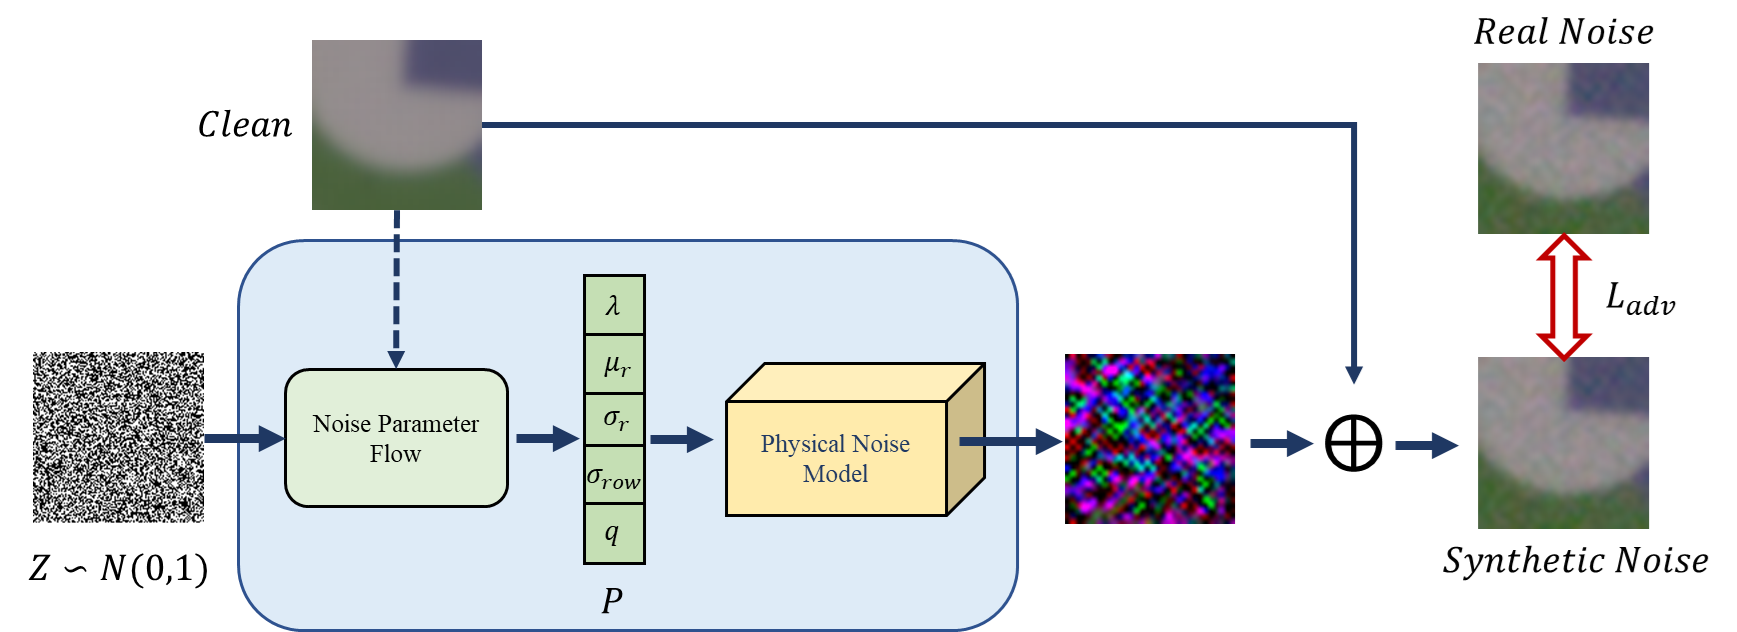
\includegraphics[width=1.0\textwidth]{imgs/noisemodeling.pdf}
	\caption{本文提出的噪声建模方法的结构。}
	\label{fig:noisemodeling}
\end{figure}

本文的工作从一个从高斯分布中随机采样的潜变量$\boldsymbol{z} \sim \mathcal{N}(\mathbf{0}, \mathbf{I})$开始,经过预先训练的噪声参数先验模型获取五个噪声参数$\boldsymbol{P}=\left(\lambda, \mu_r, \sigma_r, \sigma_{\text {row }}, q\right)$。通过获取噪声参数,生成的噪声可通过式\ref{noisemodel}中的物理噪声模型合成,将其添加到干净图像$C$中,得到模型合成的噪声图像$\hat{I}$。

\subsection{损失函数设计}

类似FKP模型,本文采用对抗训练来判别合成的噪声图像是否与真实世界场景足够相似。为了更好地提取噪声图像的特征,本文使用了PatchGAN架构\cite{patchgan}作为对抗训练的判别器,引入了一种稳健的度量方法,包括图像清晰度和结构相似性作。整个模型的优化通过对抗损失函数进行优化:
\begin{equation}
	\mathcal{L}_{a d v}=-\mathbb{E}_I[\log D(I)]-\mathbb{E}_{\boldsymbol{z}}[\log (1-D(G(\boldsymbol{z})))]
\end{equation}
其中$I$是真实捕获的噪声图像。

在噪声建模训练过程中,由于预训练的噪声参数流模型是固定的,因此实际优化参数是潜变量$\boldsymbol{z}$。通过搜索最优的潜变量$\boldsymbol{z}$,可以找到对于特定数据集最合适的噪声参数。在噪声生成阶段,有了优化的$\boldsymbol{z}$和干净的图像$C$,可以通过预训练的噪声参数流模型生成大量的噪声图像。通过结合基于流的参数先验,所提出的噪声建模方法可以根据特定的相机传感器适应各种物理噪声模型,有助于提高图像去噪质量。


